\documentclass[prez_parietal.tex]{subfiles}
\begin{document}


%========================================================================
\section{Studying physiological signals}
%========================================================================
%------------------------------------------------------------------------
\subsection{Motivations}
%------------------------------------------------------------------------

\begin{frame}{Studying brain activity through electromagnetic signals}
\begin{itemize}
    \item Brain (electrical) activity produces an electromagnetic field.
    \item This can be measured with EEG or MEG.
\end{itemize}

\begin{columns}[T]
    \column{.5\textwidth}
    \centering
    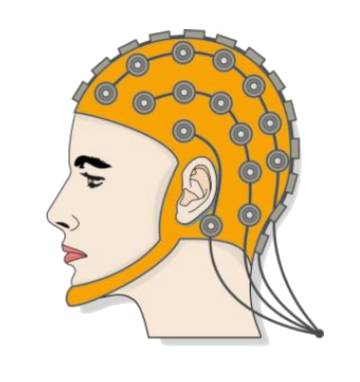
\includegraphics[height=6em]{eeg}\hskip4em
    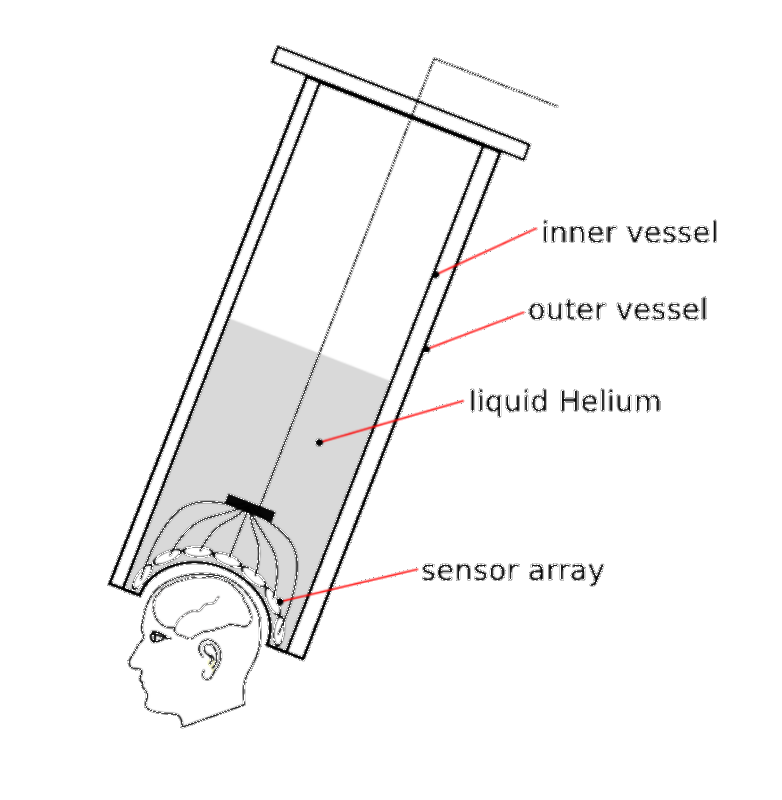
\includegraphics[height=6em]{meg}\\
    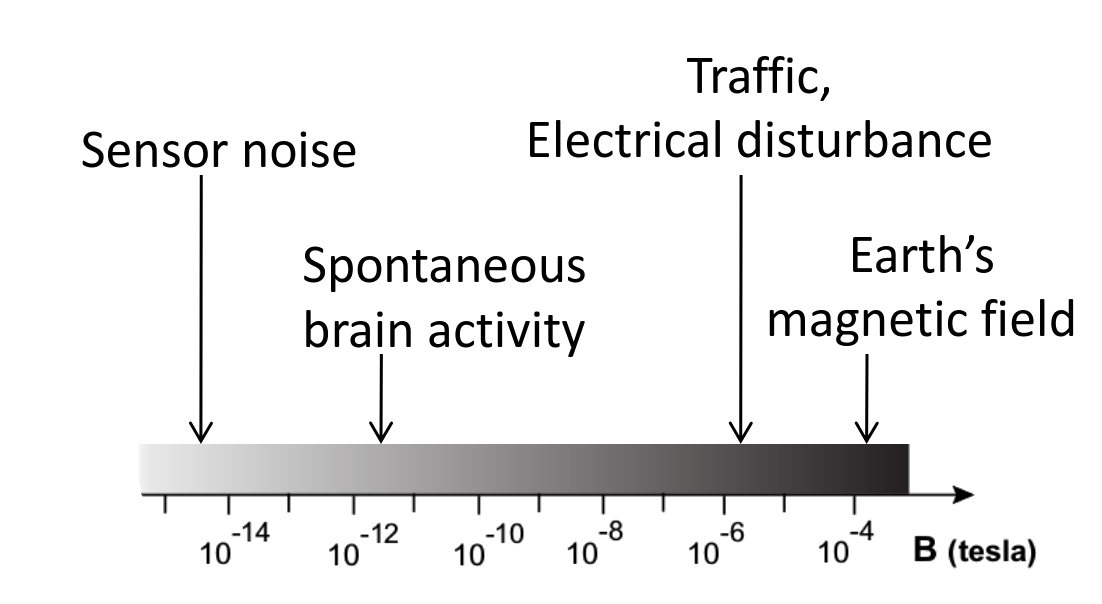
\includegraphics[height=8em]{scale_electro}
    \column{.5\textwidth}
    \vskip3em
    \hskip2em
    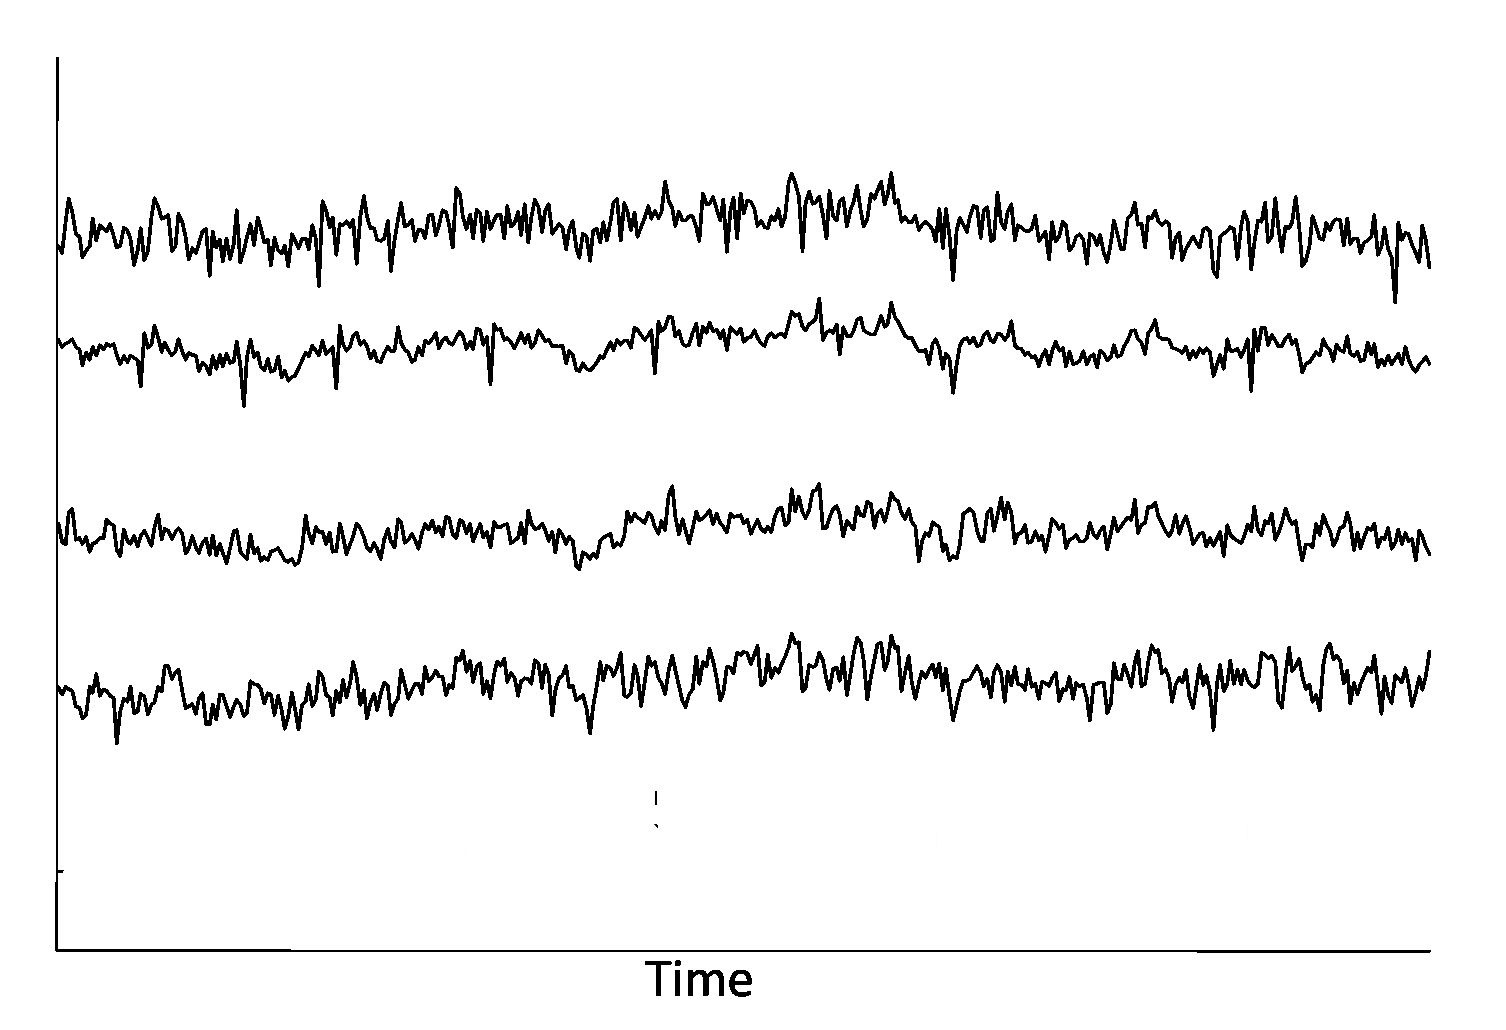
\includegraphics[height=8em]{multivariate_eeg}
\end{columns}
\end{frame}

\begin{frame}{Goal: Study Oscillation in Neural Data}

\textbf{}Oscillations are believed to play an important role in cognitive functions.\\[3em]
Many studies rely on Fourier or wavelet analyses:\\[.5em]
\begin{itemize}\itemsep1em
\item Easy interpretation,
\item Standard analysis \eg{} canonical bands alpha, beta or theta.\\\mycite{buzsaki2006rhythms}
\end{itemize}

\end{frame}

\begin{frame}{Goal: Study Oscillation in Neural Data}

However, some brain rhythms are not sinusoidal, \eg{} mu-waves.\\\mycite{hari2006action}\\
\hskip5em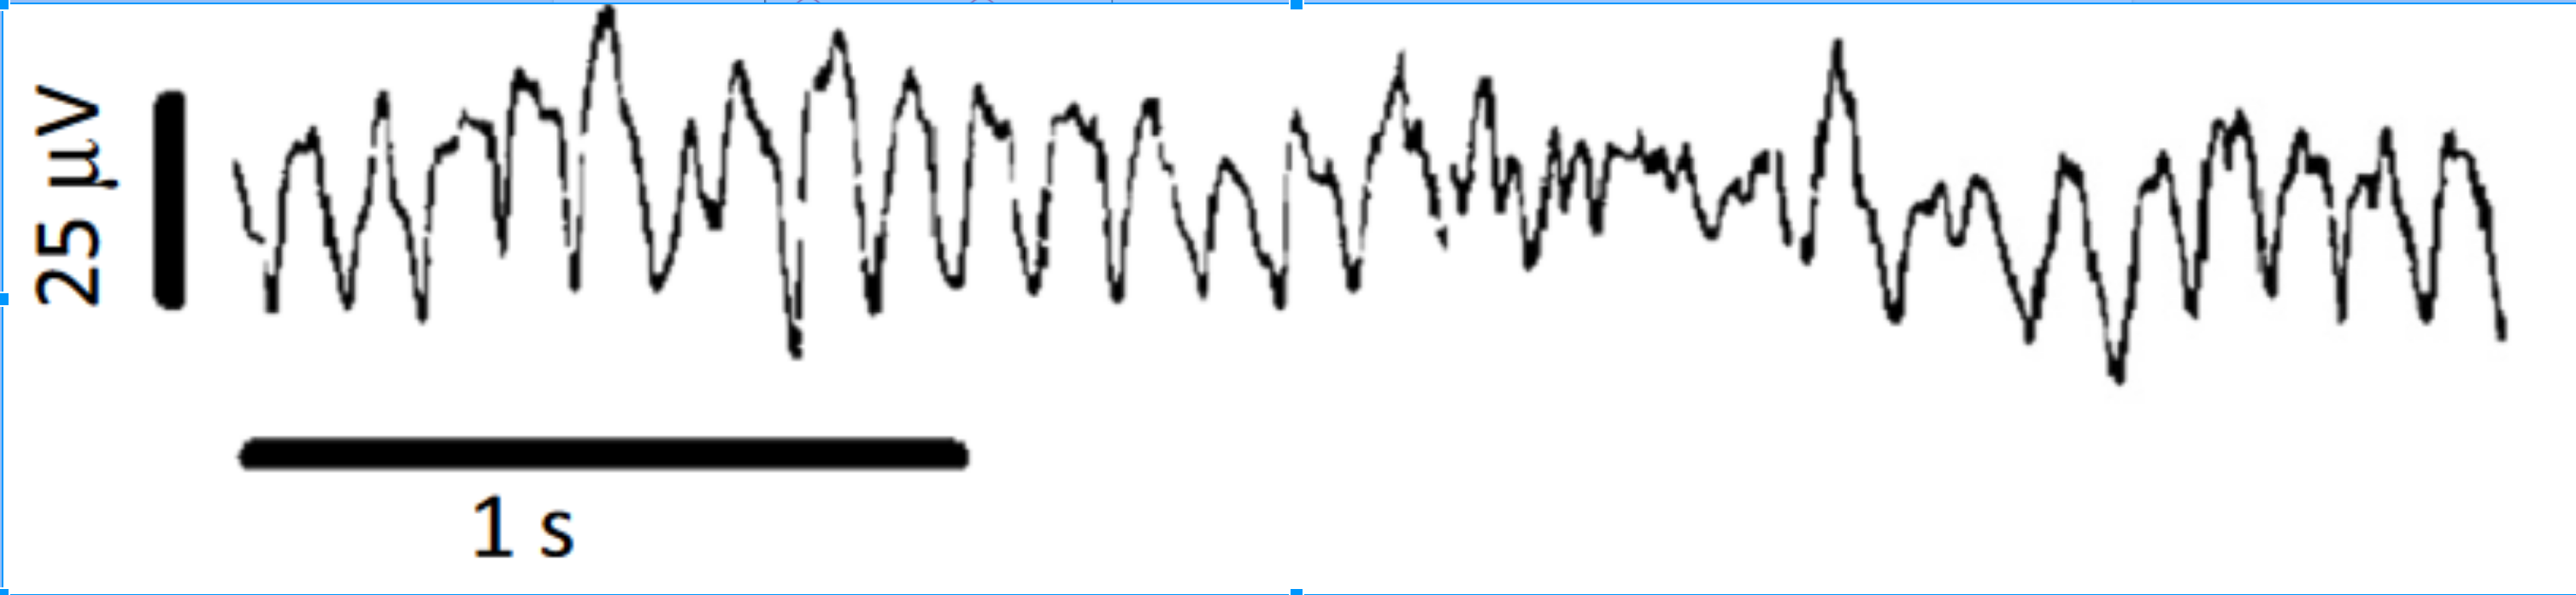
\includegraphics[width=.7\textwidth]{waveform}\\
and filtering degrades waveforms\\
\hskip8em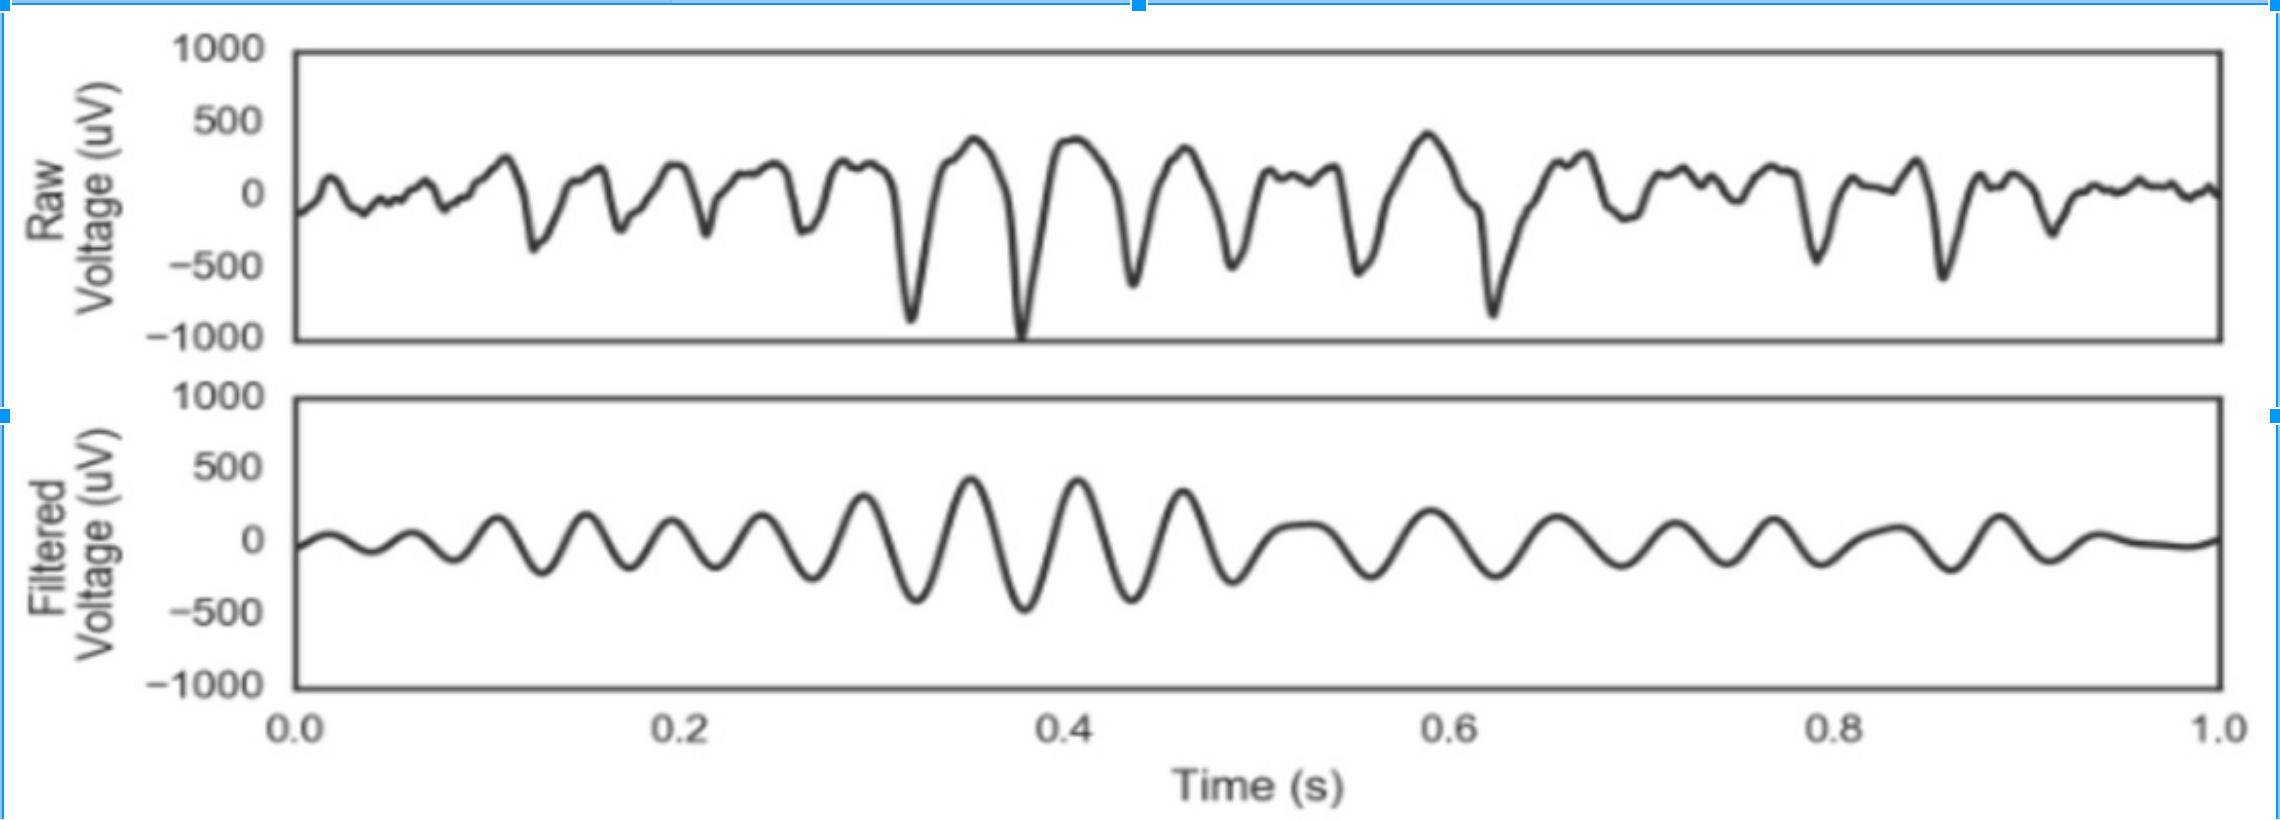
\includegraphics[width=.5\textwidth]{filtering_brain}


\strongpoint{Can we do better with data-driven approach?}
\end{frame}


\begin{frame}{Signals from human walking}
\centering
\vskip1em
\begin{tabular}{m{8em} m{20em}}
    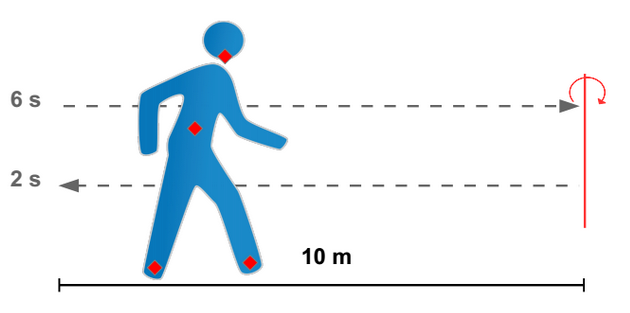
\includegraphics[width=.3\textwidth]{exo_marche}
    \raisebox{-.5\height}{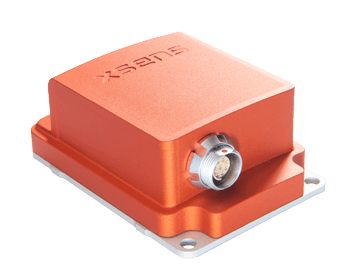
\includegraphics[width=.15\textwidth]{xsens}} $\substack{\text{Inertial}\\\text{captor}}$ &
    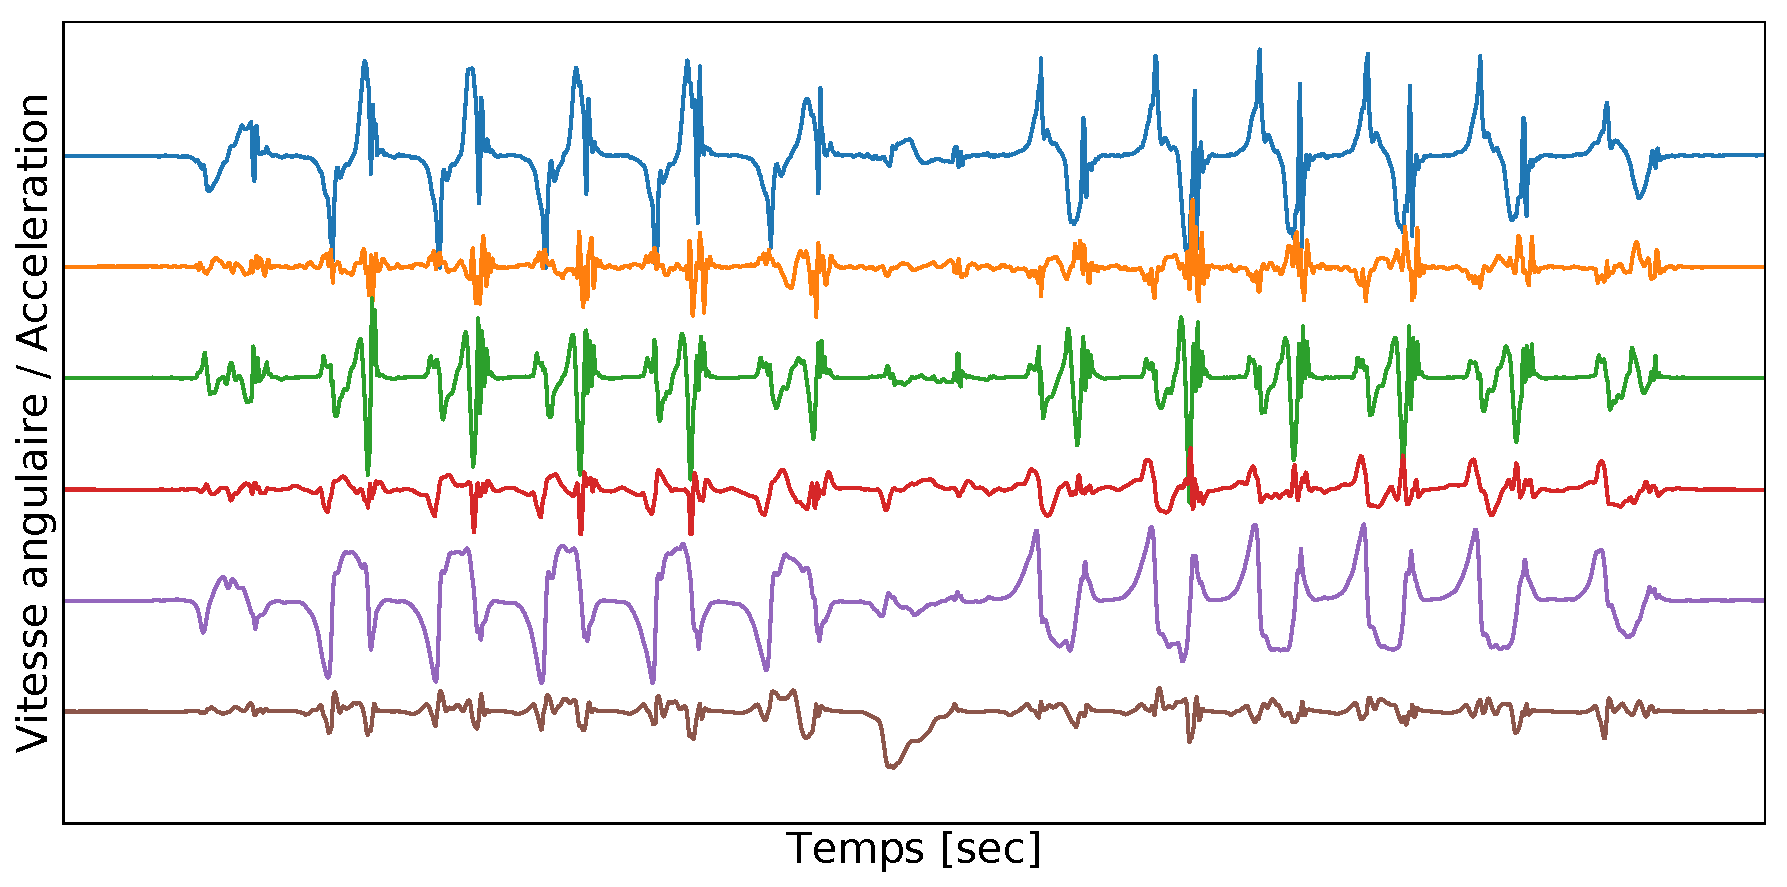
\includegraphics[width=.6\textwidth]{accelero}
\end{tabular}
\vskip1em
\begin{itemize}
    \item Shift invariant patterns linked to steps,
    \item Manual segmentation of the signal is expensive.
\end{itemize}
\strongpoint{Can we do better with data-driven approach?}

\end{frame}


%------------------------------------------------------------------------
\section{Convolutional representations}
%------------------------------------------------------------------------

\parttitleframe{}


\begin{frame}[t]
\frametitle{Model}
    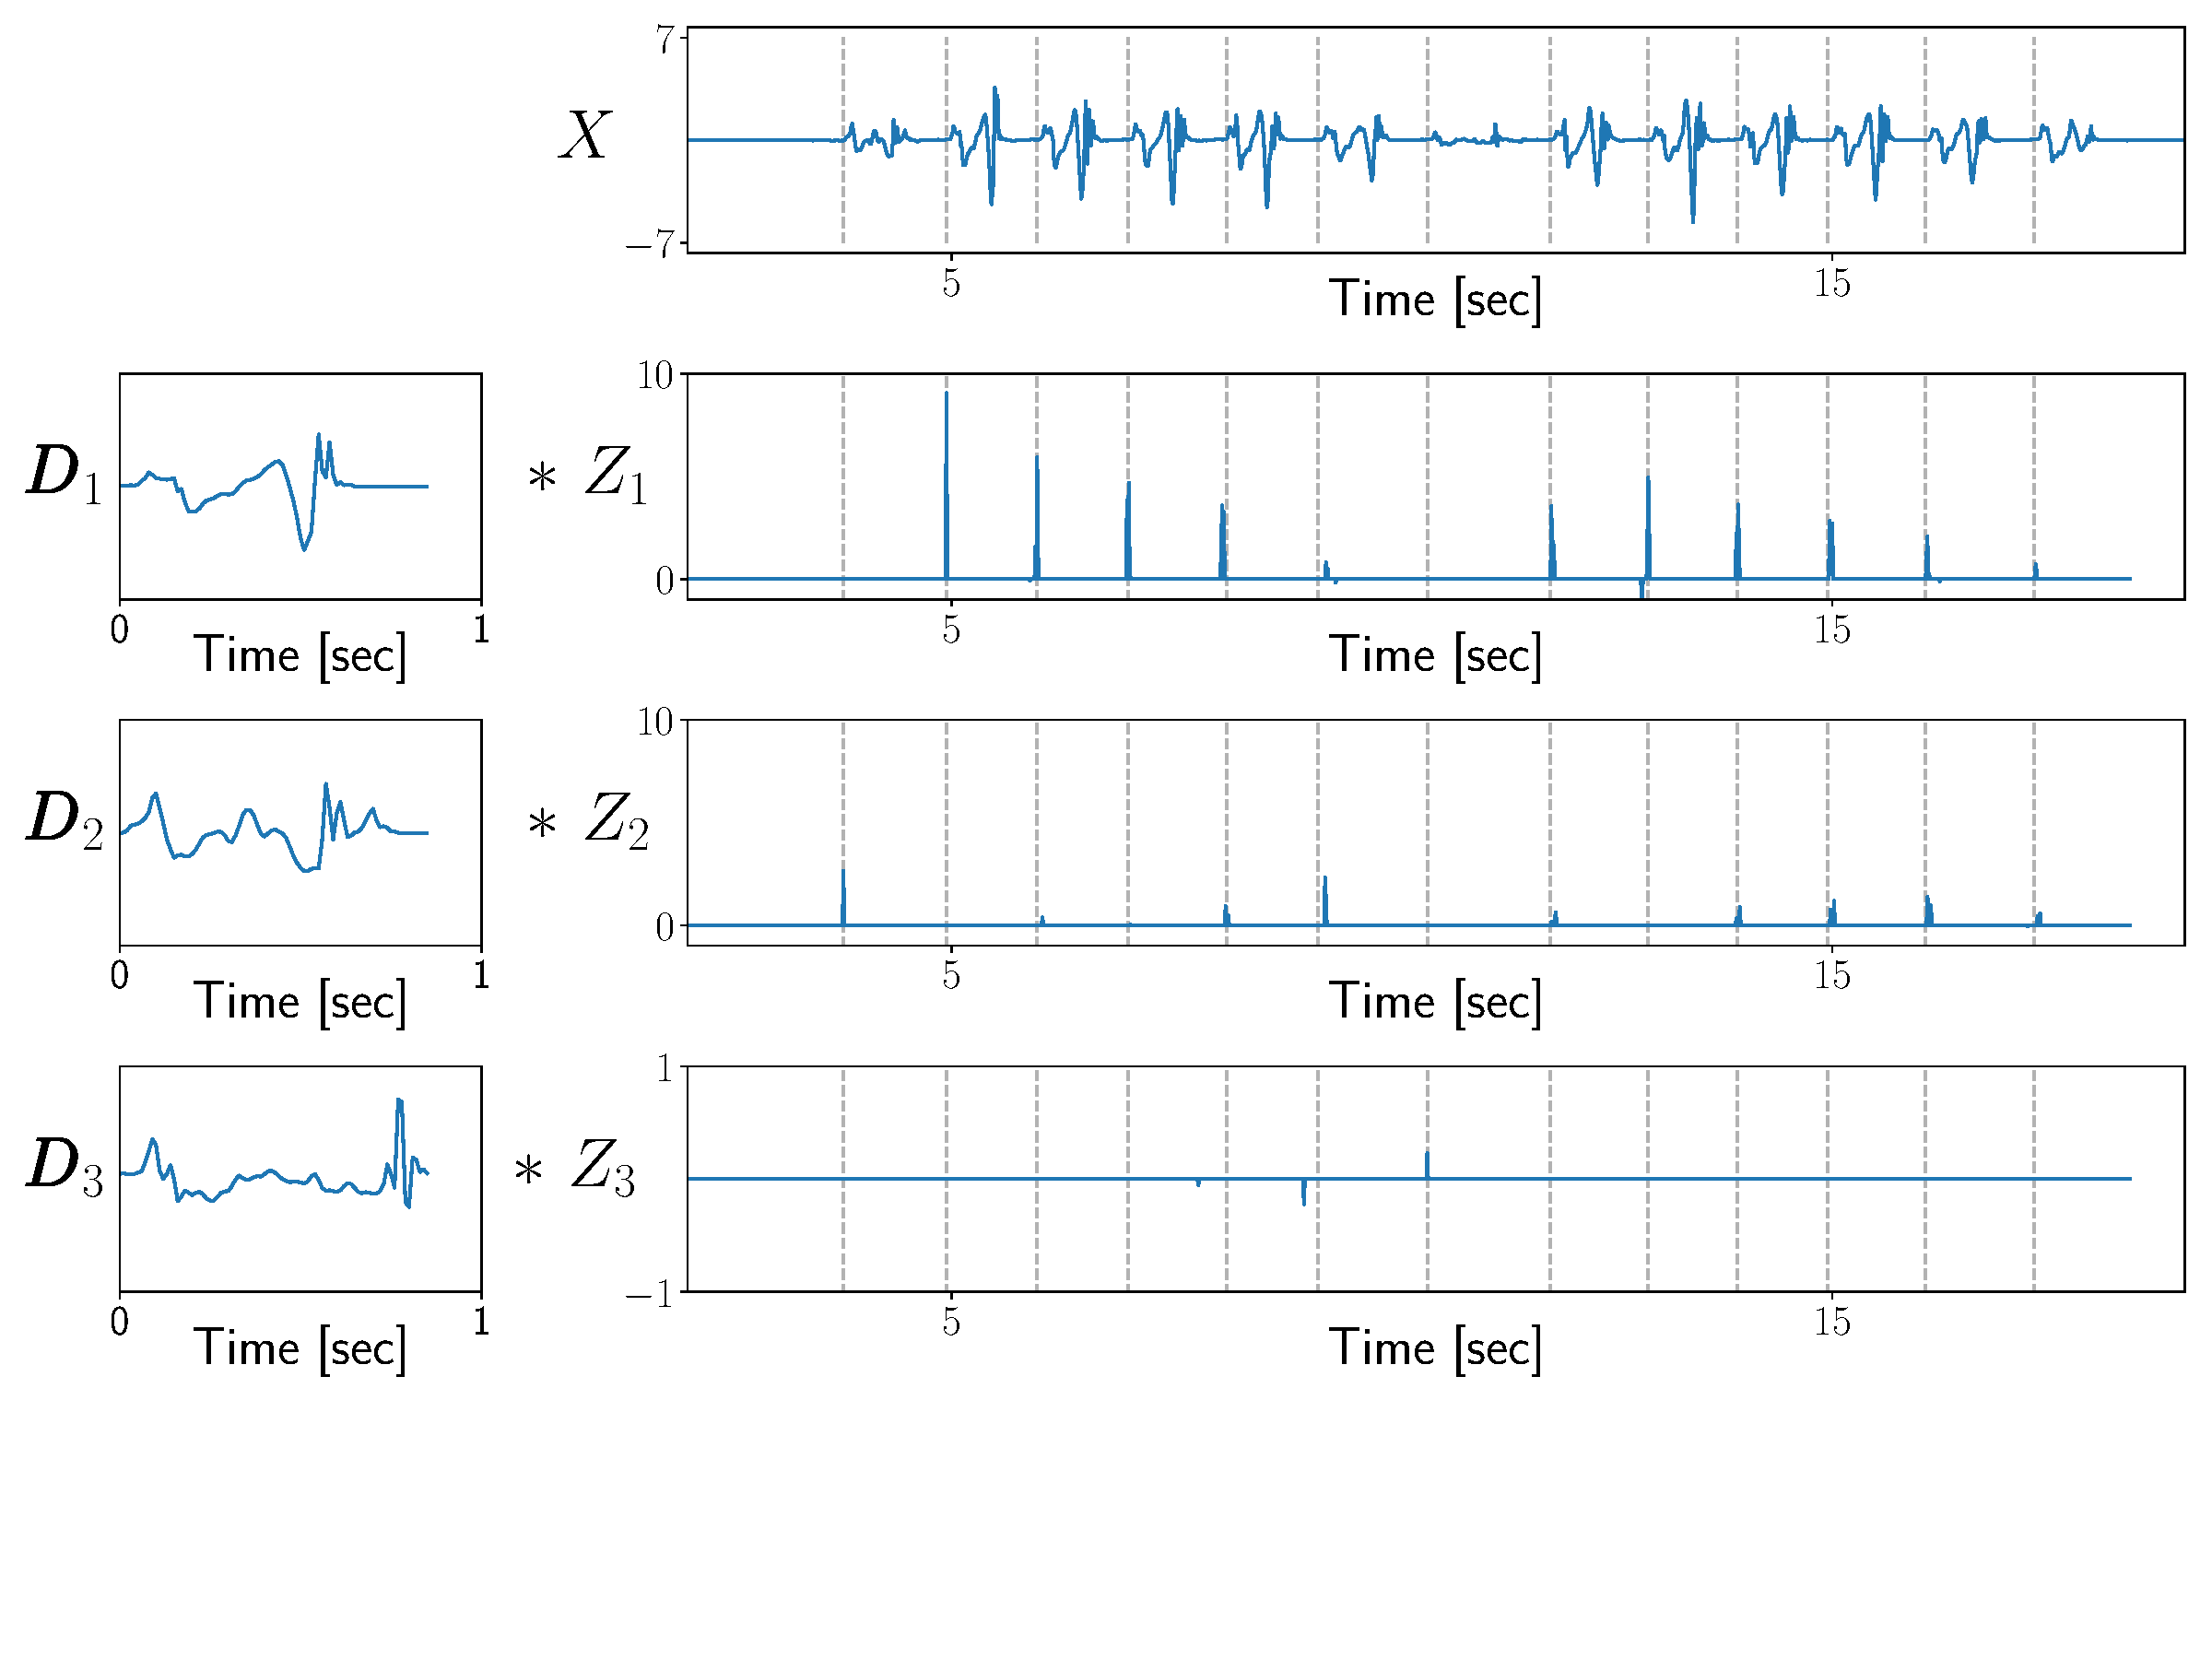
\includegraphics[width=.9\textwidth]{csc_explain}
\end{frame}

\begin{frame}[t]
\frametitle{Notation}
    \textbf{Sparse Convolutional model:}
	\begin{align*}
		X[t] & = \sum_{k=1}^K (\pmb D_k*Z_k)[t] + \mathcal E[t]
	\end{align*}
	\vskip.5em
	with \makebox[1em]{$Z$} sparse. {\color{gray} Few of its coefficients are non-zero.}
    \vskip1em
    \begin{itemize}\itemsep1em
        \item $X$ is a signal of length $T$
        \item $\mathcal E$ is a noise signal of length $T$ 
        \item $\pmb D$ is a set of $K$ patterns of length $W$
        \item $Z$ is a signal of length $L = T-W+1$ in $\Rset^K$ 
    \end{itemize}
\end{frame}

%------------------------------------------------------------------------
\subsection{Convolutional dictionary Learning}
%------------------------------------------------------------------------
\begin{frame}[t]
\frametitle{Convolutional Dictionary Learning}
Dictionary learning optimization problem for $\{X^{[n]}\}_{n=1}^N$ 
\[\hskip-2em\begin{split}
	(Z^*, \pmb D^*) = \argmin_{Z, \pmb D}\frac{1}{N}\sum_{n=1}^N
			\underbrace{\| X^{[n]} - \sum_{k=1}^K\pmb D_k *  Z_k^{[n]}\|_2^2
						}_{E(Z) \text{ data fit}}\\
			+ \underbrace{\lambda\| Z^{[n]}\|_1 + \textbf{1}_{\Omega}(D)
						}_{\text{penalizations}}
\end{split}\]
with a convex constraint set $\Omega$ and a regularization parameter $\lambda > 0$.\\
Classic constraint sets $\Omega$ are the $\ell_2$-ball or sphere.\\[1.5em]
This problem is bi-convex and an approximate solution is obtained through \textbf{alternate minimization}. \mycite{Engan1999, Grosse2007}
\end{frame}

\begin{frame}[t]
\frametitle{$\pmb D$-step: Dictionary updates}
$\rightarrow Z$ fixed, update $\pmb D$
\[
	\pmb D^* = \argmin_{\pmb D}\frac{1}{N}\sum_{n=1}^N
			\| X^{[n]} - \sum_{k=1}^K\pmb D_k *  Z_k^{[n]}\|_2^2
				+ \textbf{1}_{\Omega}(D)
\]
\vskip1.5em
%
\underline{\textbf{Related Algorithms:}}\\[.5em]
\begin{itemize}\itemsep.5em
	\item Proximal Gradient Descent (PDG) \mycite{Rockafellar1976}
	\item Accelerated PGD \mycite{Nesterov1983}
	\item Block Coordinate Descent \mycite{Mairal2010}
	\item Alternated Direction Method of Multiplier (ADMM)\\\mycite{Gabay1976}
\end{itemize}
\end{frame}

\begin{frame}[t]
%\vskip-1em
\frametitle{$Z$-step: Sparse coding}
$\rightarrow \pmb D$ fixed, update $Z$
\[
	Z^{[n],*} = \argmin_{Z^{[n]}}\| X^{[n]} - \sum_{k=1}^K\pmb D_k *  Z_k^{[n]}\|_2^2
			+ \lambda\| Z^{[n]}\|_1
\]
\strongpoint{Independent for each $n\in\llbracket1, N\rrbracket$}
\vskip1em
%
\underline{\textbf{Related Algorithms:}}\\[.5em]
\begin{itemize}%\itemsep.5em
	\item Iterative Soft-Thresholding Algorithm (ISTA)\\\mycite{Daubechies2004}
	\item Fast ISTA \\\mycite{Beck2009}
	\item Alternated Direction Method of Multiplier (ADMM)\\\mycite{Gabay1976}
	\item Coordinate Descent (CD) \\\mycite{Friedman2007}
\end{itemize}

	
\end{frame}

%\begin{frame}
%	\frametitle{Coordinate Descent \mycite{Friedman2007}}
%	{
%	\vskip2em
%	Select a coordinate $(k, t)$ and update it to the value
%	\[
%		Z_k'[t] = \argmin_{Z_k[t]}\| X - \sum_{k=1}^K\pmb D_k *  Z_k\|_2^2
%				+ \lambda\| Z\|_1
%	\]
%	with all other coordinates fixed.
	
%	\vskip2em
%	\centering
%	\inputTikZ{1}{cd_tikz}
%	}{ISTA \mycite{Daubechies2004}}{
%	\vskip2em
%	Proximal Gradient descent for Sparse Coding:
%	\[
%		Z^{(q+1)} = \text{Sh}\left(Z^{(q)} - \alpha\nabla E(Z^{(q)}), \alpha\lambda\right)
%	\]
%	with Sh$(Z_k[t], \lambda) = \text{sign}(Z_k[t])\max(|Z_k[t]|-\lambda, 0)$.

%	\vskip2em	
%	\centering
%	\inputTikZ{1}{pgd_tikz}
%	}
%\end{frame}


%---------------------------------------------------------------------------
\subsection{Accelerating the sparse coding}
%---------------------------------------------------------------------------


\begin{frame}{Part I: Adaptive Optimization}

\vskip2em
We have to solve $N$ independent problems with a common structure $\pmb D$,\\[.5em]
\[
Z^{[n],*} = \argmin_{Z^{[n]}}\| X^{[n]} - \sum_{k=1}^K\pmb D_k *  Z_k^{[n]}\|_2^2
+ \lambda\| Z^{[n]}\|_1
\]\vskip2em
{\textbf{Can we use this structure to accelerate the resolution?}\\[1em]}
\visible<2->{
    Yes, with the Learned ISTA. \mycite{Gregor10}\\[1em]
    %
    \textbf{Why does it work?} \visible<3>{Analysis in the context of sparse coding.\\\hfill{\color{gray}(no convolution)}}\\
}
\end{frame}



\begin{frame}
\frametitle{Part II: Coordinate Descent for CSC}

	Coordinate descent only performs local updates at each iteration.
	\strongpoint{More efficient for convolutional model with long signals.}
    \vskip2.5em
    {\bf Can we improve it with the structure of our problem?}
    \vskip1em
    Improving CD efficiency using the convolutional structure of the dictionary:
	\begin{itemize}\itemsep.5em
		\item Locally Greedy Coordinate Descent.
		\item Asynchronous and distributed algorithm.
	\end{itemize}


\end{frame}




\biblio{}
\end{document}